\chapter{Algebra}\label{app:algebra}
\subsection{Formulas and subalgebras}
We are in a territory where we are assuming very little about our addition 
so that we leave open the possiblity of applying the ideas of tensors broadly.
This already included examples where the data we add include things like vector spaces,
and there is no ``set of all vector spaces''.  In fact sets themselves are a bit 
of mismatch with algebra.  This causes no trouble.  Algebra predates sets 
(think of Boolean, Heyting and de Morgan algebra) and outlasts sets (think 
of categories).  If this makes you uncomfortable you should note that programming 
is in the same boat.  It describes logic outside of sets all the time.
So what is algebra without sets?  Well what is math without sets! 
It takes a step back and becomes all about language.  In otherwords 
it is time to go back to grammar school.

We want additive structures so we use $+$ and we want that be $x+y$, because 
at least for math 
styles like $+x~y$ or \code{add(x,y)} are not our preference.
To feel sophisticated about this we could report that we have the following 
grammar:
\begin{center}
\begin{lstlisting}
<A>::= (<A>+<A>) | 0
\end{lstlisting}   
\end{center}
where $|$ indicates ``or'' and so we can add or use $0$.  If we do not want 
$0$ in our addition we just remove it; likewise, if wish to add something like 
negatives we can add this as well as in the following.
\begin{center}
\begin{lstlisting}
<An>::= (<AN>+<AN>) | 0 | -<AN>
\end{lstlisting}   
\end{center}


We will want some formulas.  So we add variables, 
for examples to add $X=\{x,y,z\}$ as variables we use
\begin{center}
\begin{lstlisting}
   <X> ::= x | y 
<A<X>> ::= <X> | 0 |(<A<X>>+<A<X>>)      
\end{lstlisting}
\end{center}


Strings $\Phi:=\Phi(X)$ that prase in this grammar are called \emph{additive formulas} 
and annotated $\Phi:\text{Fr}_{A}\langle X\rangle$.  For example 
$((x+0)+y):\text{Fr}_A\langle x,y\rangle$, 
but not $+xy$ because that does not match the pattern in the grammar.

Given an additive structure $W$ and assignment of variables $w_X:W^X$
we can substitute into a formula $\Phi(X)$ the values $w_X$ formula 
a list of operations to carry out in $W$ called \emph{evaluation} and denoted 
$\Phi(w_X)$.  For example $\Phi(x,y)=((x+0)+y)$ and $W=\mathbb{N}$ then 
$\Phi(2,3)=((2+0)+3)=5$.  

Now given an additive algebra $W$ and a function $S:I\to W$, then 
the evaluations $\Phi(s_*)$ are said to have type 
\begin{align*}
    \text{Fr}_{+,0}\langle S\rangle 
\end{align*}
We say that $\text{Fr}_{+,0}\langle S\rangle$ is the subalgebra generated 
by $S$.

\subsection{Congruence, quotients, \& homomorphisms}
Algebra is the study of equations with variables, e.g.\ $x^2+1=0$.  
The most general form of algebra should allow every symbol to vary.  
So we can replace $+$ one day with addition of decimal numbers, 
the next day $+$ is addition of complex.  Later we are adding matrices
or polynomails etc.  The $+$ is changing.  But so too is the $=$. 
Equality of decimals is not equality of matrices.  The theory of 
changing equality is Noether's Isomorphism theorem.  To get there let 
us recall an even more basic resonance.

\begin{theorem}[Resonance Theorem]
    In a calculus of constructions
    \begin{center}
        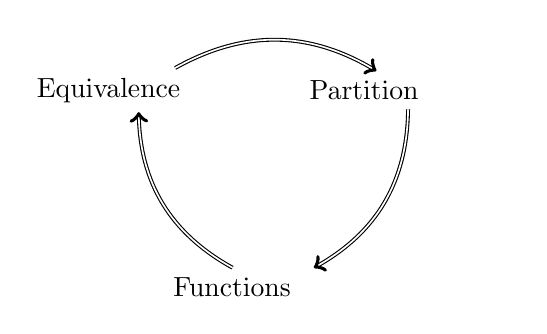
\begin{tikzpicture}
            \node[text width=1in] (EQ) at (150:2) {Equivalence};
            \node[text width=1in] (Part) at (30:2) {Partition};
            \node[text width=1in] (Fib) at (270:1.5) {Functions};

            \draw (EQ) edge[->, double, bend left] (Part);
            \draw (Part) edge[->, double, bend left] (Fib);
            \draw (Fib) edge[->, double, bend left] (EQ);
        \end{tikzpicture}
    \end{center}
\end{theorem}

Now we add algebra to the data and select those equivalence relations that respect the algebra.
Equivalence relations that respect algebra are called \emph{congruences}.
By convention a congruence relation $R$ is denoted as 
\[  
    a\equiv\acute{a}\pod{R}
\]
where $R$ is the name of the congruence.
\begin{example}
    In a $\{+,0,-\}$-algebra,
    \[
        \begin{array}{crcl}
            & a & \equiv & \acute{a} \pod{R}\\
        + &  b & \equiv & \acute{b} \pod{R}\\
        \hline 
            & a+b & \equiv & \acute{a}+\acute{b}\pod{R}
        \end{array}
        \qquad 
        \begin{array}{rcl}
            \\
            \\
        \hline 
            0 & \equiv& 0 \pod{R}
        \end{array}
        \qquad 
        \begin{array}{crcl}
            \\
        -   & a & \equiv & \acute{a} \pod{R}\\
        \hline 
            &  -a & \equiv & -\acute{a} \pod{R}
        \end{array}
    \]
    Of course operators that depend on no parameters---0-valent operators---are 
    trivially respected by all equivalence relations, but we include these 
    in the list to make it clear that every operator is being considered.
\end{example}

A partition $\{[a]\mid a\in A\}$ of an algebra that respects the operations is called a \emph{quotient}.
For instance for a $\{+,0,-\}$-algebra the partition would mean the following are well-defined.
\begin{align*}
    [a]+[b] & = [a+b] 
    & 
    [0] & = [0] 
    &
    -[a] & = [-a].
\end{align*}
By convention, quotients $\mathcal{P}$ are denoted $A/\mathcal{P}$ and the classes $[a]$, which we denote 
by $a/\mathcal{P}$, are called \emph{cosets} (even when they are not sets).

Finally a function $\varphi:A\to B$ between algebras that respects operations of (homogeneous) algebra $A$ will called a 
\emph{homomorphism} and to complete the example here is what respect means for $\{+,0,-\}$-algebras.
\begin{align*}
    \varphi(a+\acute{a}) & = \varphi(a)+\varphi(\acute{a})
    & 
    \varphi(0) & = 0
    &
    \varphi(-a) & = -\varphi(a).
\end{align*}
Now we update the resonance to match.

\begin{theorem}[Noetherian Resonance]
    In a Martin-L\"of typed algebra
    \begin{center}
        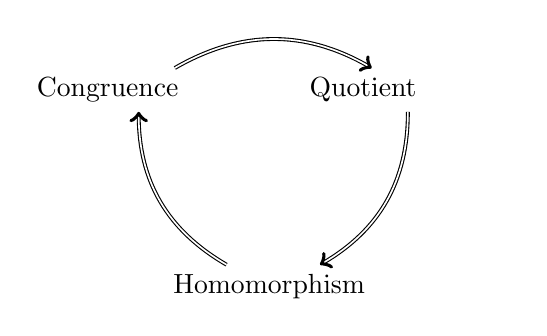
\begin{tikzpicture}
            \node[text width=1in] (EQ) at (150:2) {Congruence};
            \node[text width=1in] (Part) at (30:2) {Quotient};
            \node[text width=1in] (Fib) at (270:1.5) {Homomorphism};

            \draw (EQ) edge[->, double, bend left] (Part);
            \draw (Part) edge[->, double, bend left] (Fib);
            \draw (Fib) edge[->, double, bend left] (EQ);
        \end{tikzpicture}
    \end{center}
\end{theorem}
\begin{proof}
    From congruences to quotients use:  
    \begin{center}
        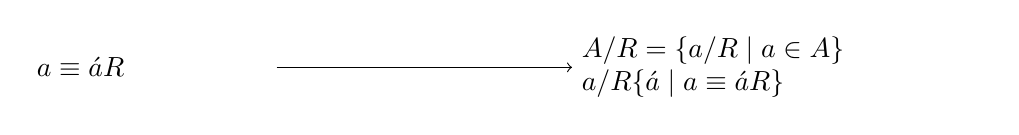
\begin{tikzpicture}
            \node[text width=1.15in] (EQ) at (0,0) {$a\equiv \acute{a}\pod{R}$};
            \node[text width=2in] (Part) at (8,0) {$A/R=\{a/R\mid a\in A\}$\\ $a/R\defeq \{\acute{a}\mid a\equiv \acute{a}\pod{R}\}$};
            \draw (EQ) edge[->, ] (Part);
        \end{tikzpicture}
    \end{center}
    
    From quotients to homomorphisms use:  
    \begin{center}
        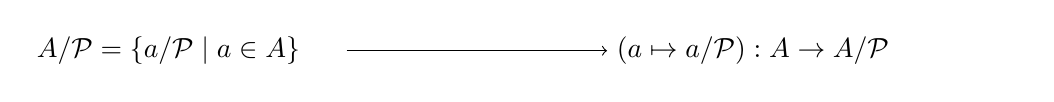
\begin{tikzpicture}
            \node[text width=1.5in] (EQ) at (0,0) {$A/\mathcal{P}=\{a/\mathcal{P}\mid a\in A\}$};
            \node[text width=2in] (Part) at (8,0) {$(a\mapsto a/\mathcal{P}):A\to A/\mathcal{P}$};
            \draw (EQ) edge[->, ] (Part);
        \end{tikzpicture}
    \end{center}

    From homomorphism to congruence use kernels.
    \begin{center}
        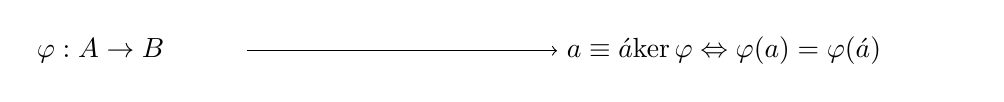
\begin{tikzpicture}
            \node[text width=1in] (EQ) at (0,0) {$\varphi:A\to B$};
            \node[text width=2in] (Part) at (8,0) {$a\equiv \acute{a} \pod{\ker \varphi} \Leftrightarrow \varphi(a)=\varphi(\acute{a})$};
            \draw (EQ) edge[->, ] (Part);
        \end{tikzpicture}
    \end{center}

\end{proof}

